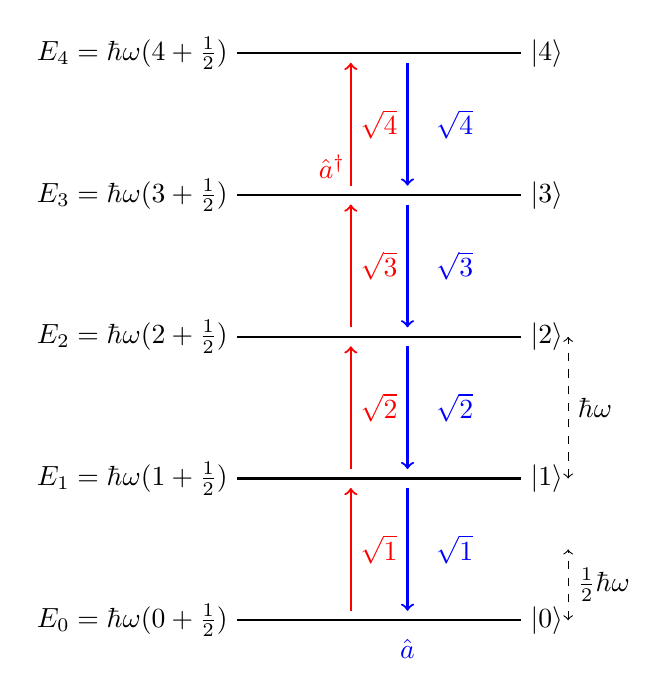
\begin{tikzpicture}[scale=1.2]
	% Niveles de energía
	\foreach \n in {0,1,2,3,4} {
		\draw[thick] (0,\n*1.5) -- (3,\n*1.5);
		\node[left] at (0,\n*1.5) {$E_{\n} = \hbar\omega(\n + \frac{1}{2})$};
		\node[right] at (3,\n*1.5) {$|{\n}\rangle$};
	}

	% Flechas de creación (rojas, hacia arriba)
\foreach \n in {0,1,2,3} {
	\pgfmathtruncatemacro{\m}{\n+1}
	\draw[->,red,thick] (1.2,\n*1.5+0.1) -- (1.2,\m*1.5-0.1);
	\node[red,right] at (1.2,\n*1.5+0.75) {$\sqrt{\m}$};
}
\node[red] at (1,4.8) {$\hat{a}^\dagger$};
		
		
		
		
		% Flechas de aniquilación (azules, hacia abajo)
	\foreach \n in {1,2,3,4} {
		\pgfmathtruncatemacro{\m}{\n-1}
		\draw[->,blue,thick] (1.8,\n*1.5-0.1) -- (1.8,\m*1.5+0.1);
		\node[blue,right] at (2,\n*1.5-0.75) {$\sqrt{\n}$};
	}
	\node[blue] at (1.8,-0.3) {$\hat{a}$};
	
	% Energía de punto cero
	\draw[<->,dashed] (3.5,0) -- (3.5,0.75);
	\node[right] at (3.5,0.375) {$\frac{1}{2}\hbar\omega$};
	\draw[<->,dashed] (3.5,1.5) -- (3.5,3);
	\node[right] at (3.5,2.25) {$\hbar\omega$};
	
\end{tikzpicture}
